\section{Introduction}

\subsection{History}
The idea that \ac{LAMs} could be used for regional studies was originally proposed by \citet{Dickinson_89} and \citet{Giorgi_90}. This idea was based on the concept of one-way nesting, in which large scale meteorological fields from \ac{GCM} runs provide initial and time-dependent meteorological \ac{LBCs} for high resolution \ac{RCM} simulations, with no feedback from the \ac{RCM} to the driving \ac{GCM}.

The first generation NCAR \ac{RegCM} was built upon the \ac{NCAR}-\ac{PSU} \ac{MM4} in the late 1980s \citep{Dickinson_89,Giorgi_89}. The dynamical component of the model originated from the \ac{MM4}, which is a compressible, finite difference model with hydrostatic balance and vertical $\sigma$-coordinates. Later, the use of a split-explicit time integration scheme was added along with an algorithm for reducing horizontal diffusion in the presence of steep topographical gradients \citep{Giorgi_93,Giorgi_93b}.  As a result, the dynamical core of the \ac{RegCM} is similar to that of the hydrostatic version of \ac{MM5} \citep{Grell_94}.

For application of the \ac{MM4} to climate studies, a number of physics parameterizations were replaced, mostly in the areas of radiative transfer and land surface physics, which led to the first generation \ac{RegCM} \citep{Dickinson_89,Giorgi_90}. The first generation \ac{RegCM} included the Biosphere-Atmosphere Transfer Scheme, BATS, \citep{Dickinson_86} for surface process representation, the radiative transfer scheme of the \ac{CCM1}, a medium resolution local planetary boundary layer scheme, the Kuo-type cumulus convection scheme of \citep{Anthes_77} and the explicit moisture scheme of \citep{Hsie_84}.

A first major upgrade of the model physics and numerical schemes was documented by \citep{Giorgi_93,Giorgi_93b}, and resulted in a second generation \ac{RegCM}, hereafter referred to as \ac{RegCM2}. The physics of \ac{RegCM2} was based on that of the \ac{NCAR} \ac{CCM2} \citep{Hack_93}, and the mesoscale model \ac{MM5} \citep{Grell_94}. In particular, the \ac{CCM2} radiative transfer package \citep{Briegleb_92} was used for radiation calculations, the non local boundary layer scheme of \citep{Holtslag_90} replaced the older local scheme, the mass flux cumulus cloud scheme of \citep{Grell_93} was added as an option, and the latest version of BATS1E \citep{Dickinson_93} was included in the model.

In the last few years, some new physics schemes have become available for use in the \ac{RegCM}, mostly based on physics schemes of the latest version of the \ac{CCM}, \ac{CCM3} \citep{Kiehl_96}. First, the \ac{CCM2} radiative transfer package has been replaced by that of the \ac{CCM3}. In the \ac{CCM2} package, the effects of ${\rm H_2O}$, ${\rm O_3}$, ${\rm O_2}$, ${\rm CO_2}$ and clouds were accounted for by the model. Solar radiative transfer was treated with a $\delta$-Eddington approach and cloud radiation depended on three cloud parameters, the cloud fractional cover, the cloud liquid water content, and the cloud effective droplet radius. The \ac{CCM3} scheme retains the same structure as that of the \ac{CCM2}, but it includes new features such as the effect of additional greenhouse gases (${\rm NO_2, CH_4, CFCs}$), atmospheric aerosols, and cloud ice.
 
The other primary changes are in the areas of cloud and precipitation processes. The original explicit moisture scheme of \citet{Hsie_84} has been substituted with a simplified version because the original scheme was computationally too expensive to be run in climate mode. In the simplified scheme only a prognostic equation for cloud water is included, which accounts for cloud water formation, advection and mixing by turbulence, re-evaporation in sub-saturated conditions, and conversion into rain via a bulk autoconversion term. The main novelty of this scheme does not reside of course in the simplistic microphysics, but in the fact that the prognosed cloud water variable is directly used in the cloud radiation calculations. In the previous versions of the model, cloud water variables for radiation calculations were diagnosed in terms of the local relative humidity. This new feature adds a very important and far reaching element of interaction between the simulated hydrologic cycle and energy budget calculations. 

%Other new features in the \ac{RegCM} include improvements in the coupled lake model \citep{Small_99} and the incorporation of a tracer model with capability of radiative interactions \citep{Qian_99}.

%Finally, an important aspect of model development was the inclusion of a stretched grid 
%model configuration, by which the model horizontal resolution is relatively coarse in 
%the lateral buffer zone and increases towards the interior of the domain. Preliminary 
%experiments using an adiabatic version of the model in stretched grid mode are presented 
%by \citep{Qian_99}. However, the stretched grid option is not available with the 
%new \ac{RegCM}3 version.  

Changes in the model physics include a large-scale cloud and precipitation scheme which accounts for the subgrid-scale variability of clouds \citep{Pal_00}, new parameterizations for ocean surface fluxes \citep{Zeng_98}, and a cumulus convection scheme \citep{Emanuel_91,Emanuel_99}. Also new in the model is a mosaic-type parameterization of subgrid-scale heterogeneity in topography and land use \citep{Giorgi_03}. Other improvements in \ac{RegCM}3 involve the input data.  The USGS Global Land Cover Characterization and Global 30 Arc-Second Elevation datasets are now used to create the terrain files.  In addition, NCEP and ECMWF global reanalysis datasets are used for the intial and boundary conditions. Lastly, improvements in the user-friendliness of the model have been made.  New scripts have been included which make running the programs easier.  Also, a new website has been developed where users can freely download the entire \ac{RegCM} system, as well as all of the input data necessary for a simulation.  

The \ac{RegCM} modeling system has four components: Terrain, ICBC, \ac{RegCM}, and Postprocessor.  Terrain and ICBC are the two components of \ac{RegCM} preprocessor. Terrestrial variables (including elevation, landuse and sea surface temperature) and three-dimensional isobaric meteorological data are horizontally interpolated from a latitude-longitude mesh to a high-resolution domain on either a Rotated (and Normal) Mercator, Lambert Conformal, or Polar Stereographic projection. Vertical interpolation from pressure levels to the $\sigma$ coordinate system of \ac{RegCM} is also performed. $\sigma$ surfaces near the ground closely follow the terrain, and the higher-level $\sigma$ surfaces tend to approximate isobaric surfaces. 

Since the vertical and horizontal resolution and domain size can vary, the modeling package programs employ parameterized dimensions requiring a variable amount of core memory, and the requisite hard-disk storage amount is varied accordingly.

\subsection{The \ac{RegCM} Model Horizontal and Vertical Grid}

\begin{figure}[!]
\begin{center}
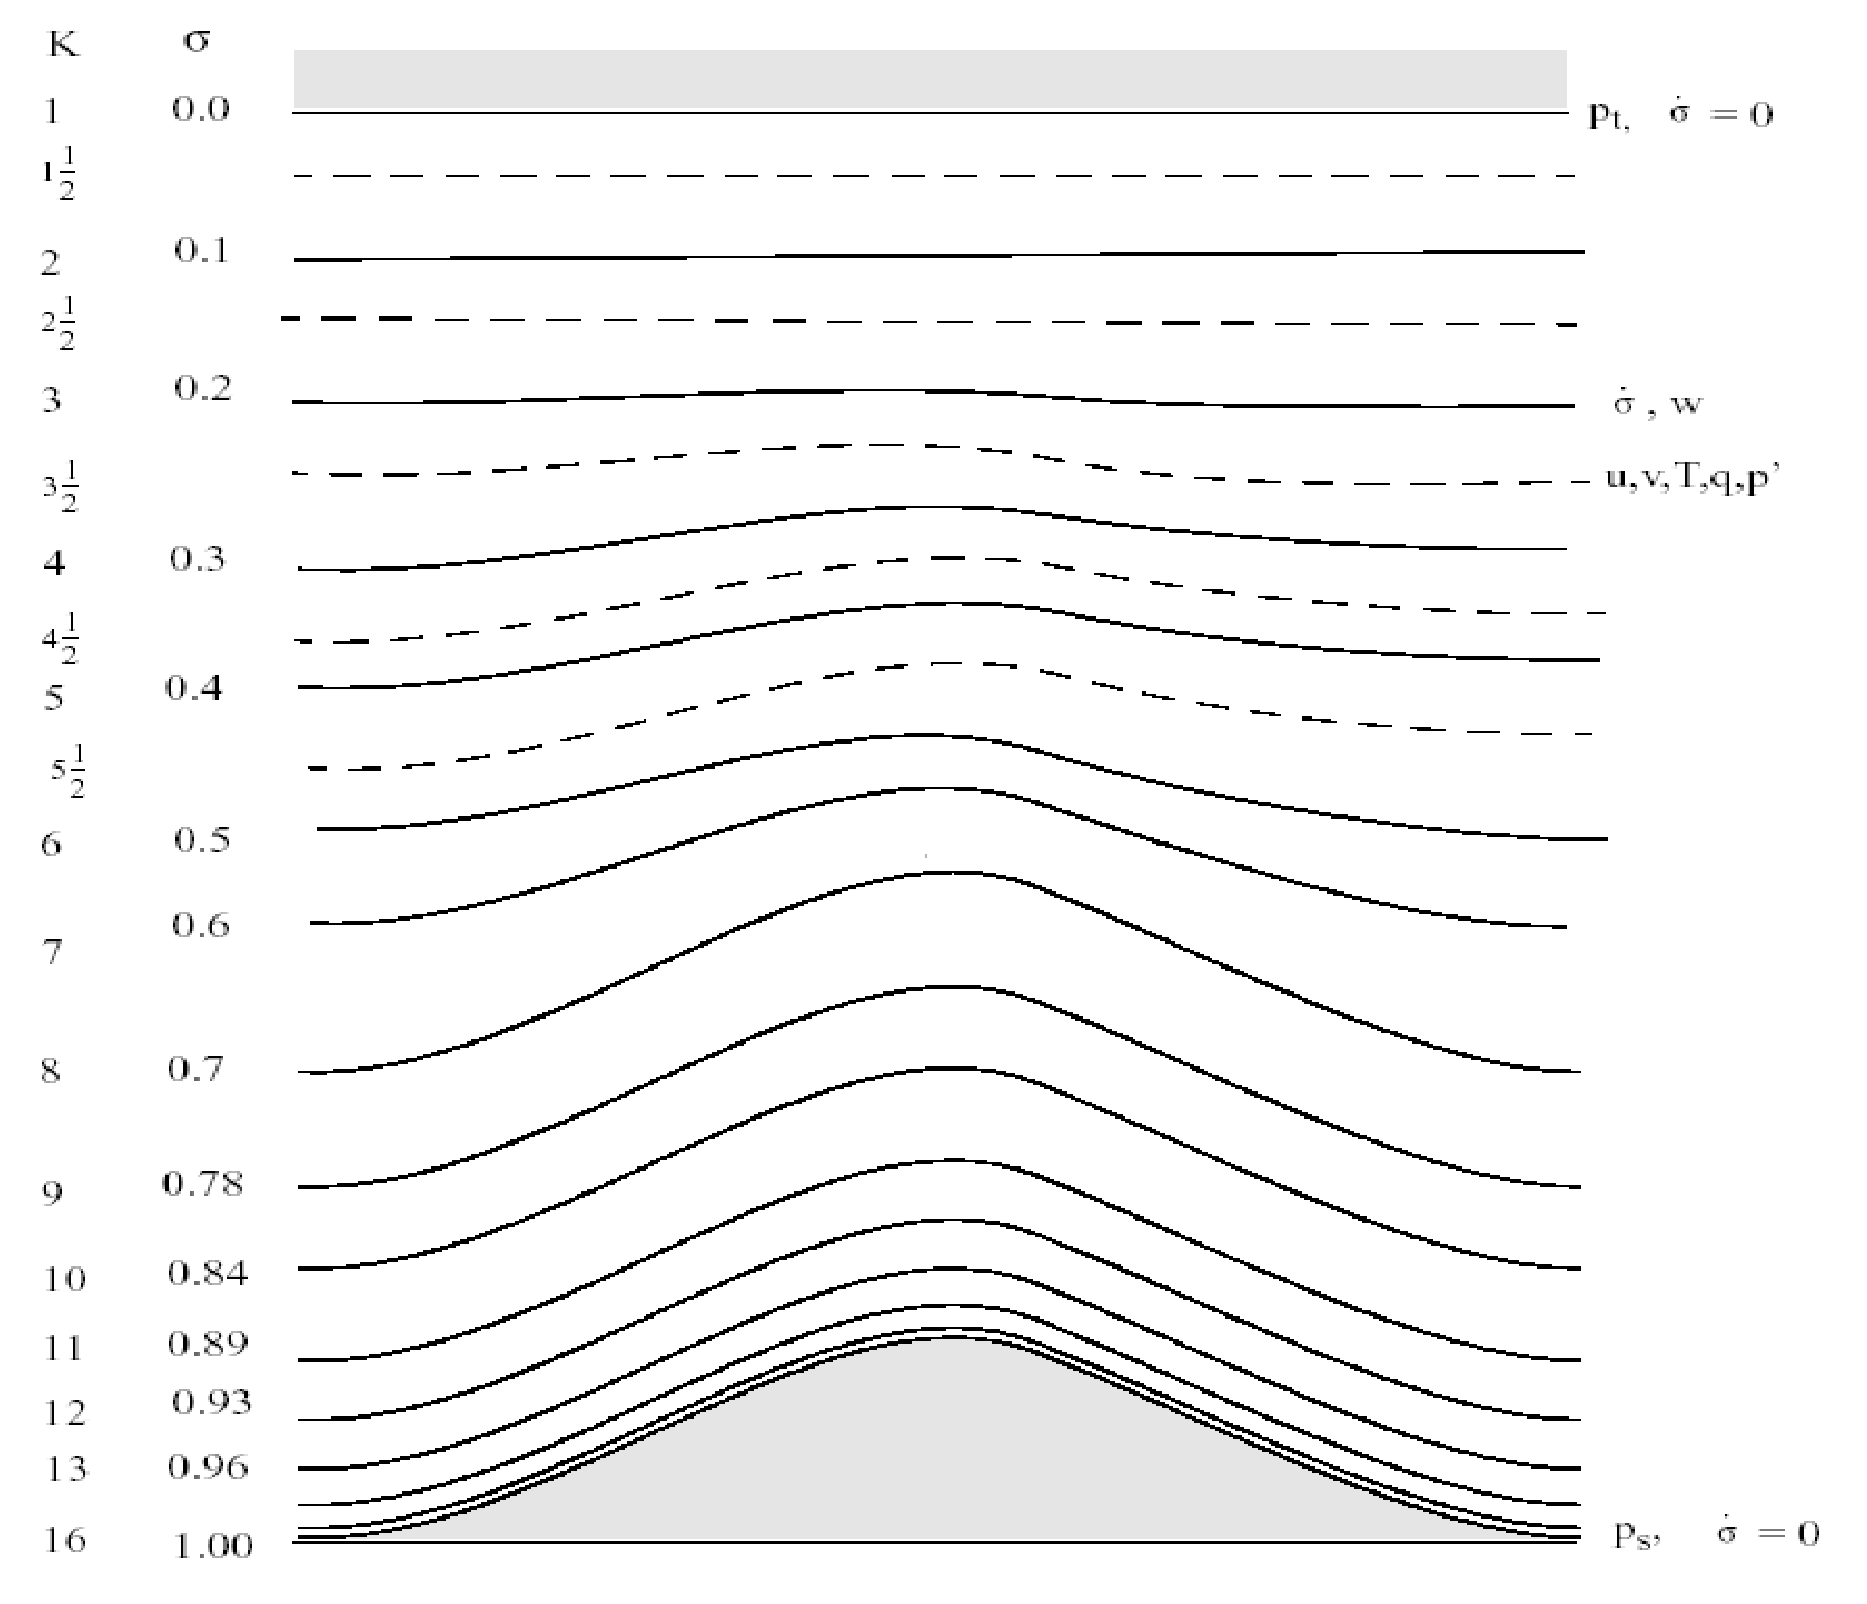
\includegraphics[scale=0.4]{sigma_levels.eps}
\caption{Schematic representation of the vertical structure of the model.  This example is for 16 vertical layers.  Dashed lines denote half-sigma levels, solid lines denote full-sigma levels. (Adapted from the PSU/NCAR Mesoscale Modeling System Tutorial Class Notes and User's Guide.)}
\label{sigma_levels}
\end{center}
\end{figure}

It is useful to first introduce the model's grid configuration. The modeling system usually gets and analyzes its data on pressure surfaces, but these have to be interpolated to the model's vertical coordinate before input to the model. The vertical coordinate is terrain-following (Figure~\ref{sigma_levels}) meaning that the lower grid levels follow the terrain while the upper surface is flatter. Intermediate levels progressively flatten as the pressure decreases toward the top of the model. A dimensionless $\sigma$ coordinate is used to define the model levels where $p$ is the pressure, $p_t$ is a specified constant top pressure, 
$p_s$ is the surface pressure.
\begin{eqnarray}
\sigma = {(p - p_t) \over (p_s - p_t)}
\end{eqnarray}

It can be seen from the equation and Figure~\ref{sigma_levels} that $\sigma$ is zero at the top and one at the surface, and each model level is defined by a value of $\sigma$. The model vertical resolution is defined by a list of values between zero and one that do not necessarily have to be evenly spaced. Commonly the resolution in the boundary layer is much finer than above, and the number of levels may vary upon the user demand.

\begin{figure}
\begin{center}
\resizebox{5.5in}{!}{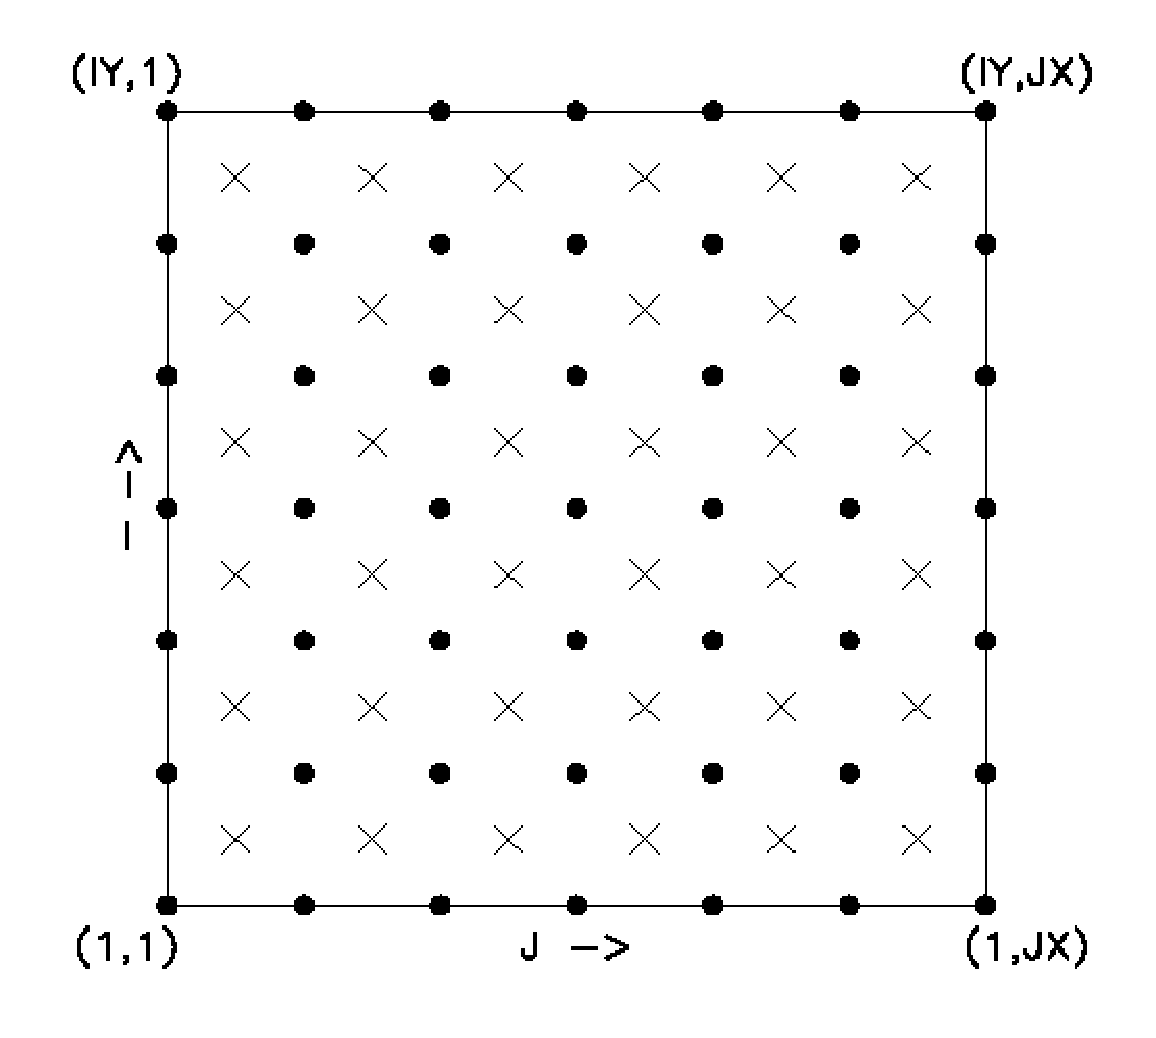
\includegraphics{grid2.eps}}
\caption{Schematic representation showing the horizontal Arakawa B-grid staggering
of the dot and cross grid points.}  \label{grid}
\end{center}
\end{figure}

The horizontal grid has an Arakawa-Lamb B-staggering of the velocity variables with 
respect to the scalar variables. This is shown in Figure~\ref{grid} where it can be seen that the scalars (T, q, p, etc) are defined at the center of the grid box, while the eastward (u) and 
northward (v) velocity components are collocated at the corners. The center points of 
grid squares will be referred to as cross points, and the corner points are dot points. 
Hence horizontal velocity is defined at dot points. Data is input to the model, the preprocessors do the necessary interpolation to assure consistency with the grid.

All the above variables are defined in the middle of each model vertical layer, referred 
to as half-levels and represented by the dashed lines in  Figure~\ref{sigma_levels}. Vertical velocity is carried at the full levels (solid lines). In defining the sigma levels it is the full levels that are listed, including levels at $\sigma$ = 0 and 1. The number of model layers is therefore always one less than the number of full sigma levels.

The finite differencing in the model is, of course, crucially dependent upon the grid 
staggering wherever gradients or averaging are represented terms in the equation.

\subsection{Map Projections and Map-Scale Factors}
The modeling system has a choice of four map projections. Lambert Conformal is 
suitable for mid-latitudes, Polar Stereographic for high latitudes, Normal Mercator for 
low latitudes, and Rotated Mercator for extra choice. The $x$ and $y$ directions in the model do not correspond to west-east and north-south except for the Normal Mercator projection, and therefore the observed wind generally has to be rotated to the model grid, and the model $u$ and $v$ components need to be rotated before comparison with observations. These transformations are 
accounted for in the model pre-processors that provide data on the model grid, and in the post-processors.  The map scale factor, $m$, is defined by \\

$m$ = (distance on grid) / (actual distance on earth)

\noindent \\
and its value is usually close to one, varying with latitude. The projections in the model preserve the shape of small areas, so that dx=dy everywhere, but the grid length varies across the domain to allow a representation of a spherical surface on a plane surface. Map-scale factors need to be accounted for in the model equations wherever horizontal gradients are used.


